% =========================================================================== %
% Preamble                                                                    %
% =========================================================================== %

\documentclass[dvipsnames, 12pt]{article}
\usepackage[utf8]{inputenc}

% Set paper geometry
\usepackage[letterpaper, margin=1.87cm]{geometry}

% Must include this before setting title and author
\usepackage{findlay}

\def\bpfcontain{\textsc{BPFContain}}

\title{\Large \bpfcontain: Towards Secure and Usable Containers with eBPF\\{\large COMP5900I Preliminary Work}}
\lhead{\bpfcontain: Towards Secure and Usable Containers with eBPF}

\author{William Findlay}
% For acmart.cls:
%\affiliation{Carleton University}
%\email{williamfindlay@cmail.carleton.ca}

% Add bibliography:
\addbibresource{ref.bib}

% To set sans serif font:
%\renewcommand{\familydefault}{\sfdefault}

% =========================================================================== %
% Document                                                                    %
% =========================================================================== %

\begin{document}

% Note from Anil:
% Final paper needs to make the case for why we shouldn't do this in a kernel
% module --- kernel module would need too much kernelspace code, eBPF is safer,
% etc.

% Title page
\maketitle
\thispagestyle{empty}

\vfill
\begin{abstract}
\noindent
\todo{Redo this abstract when I have time}
Containers are becoming an increasingly important part of the Linux ecosystem.
Containerized package managers like Snapcraft \cite{snap} and FlatPak
\cite{flatpak} enable easy distribution and dependency management for desktop
applications, while Docker \cite{docker} and Kubernetes \cite{kubernetes}
provide a framework for scaling and composing micro-services, especially in the
cloud.  While containers offer a convenient abstraction for distributing and
configuring software, they are also often used as a light-weight alternative to
heavier virtualization techniques, such as virtual machines. Thus, containers
can also be thought of as security mechanisms, implementing a form of isolation
between processes that share the resources of the underlying operating system.

Despite this clear security use case, existing container implementations do not
consider security as a primary goal, and often fall back to insecure defaults
when the host does not support the correct security abstractions. Further,
container security implementations are often complex, relying on a myriad of
virtualization techniques and security abstractions provided by the host
operating system to isolate processes and enforce least-privilege. These
security abstractions often paradoxically require elevated permissions to use in
the first place, resulting in additional security risks when applications are
able to escape confinement.

To rectify these container security issues, I present
\bpfcontain{}\footnote{\bpfcontain{} is a working title and is subject to change in the
future.}, a novel approach to containers under the Linux kernel. \bpfcontain{} is
built from the ground up as a light-weight yet secure process confinement
solution for modern applications. Implemented in eBPF, an emerging technology
for safely extending the Linux kernel, \bpfcontain{} enforces least privilege in
containerized applications without requiring any additional privileges from the
host operating system. Policies are written in a high-level language that is
designed to be readable and modifiable by end-users without requiring
significant security expertise. In this paper, I describe \bpfcontain{}'s design and
implementation, evaluate its performance and security, and discuss how it
compares with existing container solutions.

\end{abstract}
\vfill
\vfill

\clearpage

% Reset page numbering
\pagenumbering{arabic}
\setcounter{page}{1}

% Table of Contents, List of Figures, List of Tables, List of Listings
%\begingroup
%\hypersetup{linkcolor=black}
%\tableofcontents
%\newpage
%\listoffigures
%\newpage
%\listoftables
%\newpage
%\lstlistoflistings
%\newpage
%\endgroup

% Reset page numbering
\pagenumbering{arabic}
\setcounter{page}{1}

% Uncomment for 1.5 spacing:
\onehalfspacing

\section{Introduction}

\todo{Introduce the idea of containers, container security, and the need for secure containers}

\todo{Talk about \bpfcontain{} and what it does}

\todo{List contributions: container-specific LSM implementation, security-first approach to containers, least-privilege at the LSM level and hardening against kernel exploitation using kprobes}

\todo{The rest of this paper proceeds as follows...}


\section{Background}
\label{sec:background}

\subsection{The Process Confinement Problem}

The \textit{process confinement problem}, also known as the \textit{sandboxing problem}, refers to the goal of isolating a process or group of processes from the rest of the running system. In practice, this is often achieved by restricting an application's possible behaviour to its desired functionality, explicitly targeting its access to security-sensitive system resources such as files, network interfaces, and other running applications.  Despite decades of work following Lampson's \cite{lampson1973_a_note} first proposal of the process confinement problem in 1973, process confinement remains a somewhat open problem to date \cite{crowell2013_confinement_problem}.

Anderson's 1972 introduction of the reference monitor architecture \cite{anderson1973_planning_study}  has informed the design and implementation of operating system access control mechanisms for nearly five decades. As subjects request access to system resources, the kernel's reference monitor validates requests and makes policy decisions. While all commodity operating systems support at least a basic notion of access control, many implement a coarse-grained, discretionary access control mechanism that is insufficient for providing the fine-grained protection required in security-sensitive or multi-tenant environments. For additional protection, we must turn to more advanced security features offered by the operating system.

A separate yet related problem involves constructing policy languages with which to express security policy. These policy languages need to offer a careful balance of terseness and expressiveness. A policy language must be terse enough to enable human policy authorship and audit yet expressive enough to enforce least-privilege. Similarly, careful consideration is required when developing policy language abstractions. Close conformity with the system's underlying semantics may improve policy expressiveness but impact usability. Significant abstractions might similarly impact the expressiveness of the policy language.

These issues of policy enforcement and policy language design are at the heart of the process confinement problem. This paper seeks to tackle this problem from the perspective of containers and container management.

\subsection{Low-Level Isolation Techniques}
\label{subsection:low_level}

The Linux kernel supports various lower-level abstractions for implementing virtualization and enforcing least-privilege. While many of these mechanisms are insufficient for a full confinement implementation on their own, they are typically used, in \textit{combination}, by higher-level techniques such as containers (c.f.~\Cref{subsection:containers}) to achieve confinement. This section covers these low-level abstractions in detail.

%\todo{Go over each of the following subsections, since they are mostly unchanged from the literature review}

\paragraph*{Unix Discretionary Access Control}

Discretionary access control (DAC) forms the most basic access control mechanism in many operating systems, including popular commodity operating systems such as Linux, macOS, and Windows.  First formalized in the 1983 Department of Defense standard \cite{orange_book}, a DAC system partitions system objects (e.g.~files) by their respective owners and allows resource owners to grant access to other users at their discretion.  Typically, systems implementing discretionary access control also provide an exceptional user or role with the power to override discretionary access controls, such as the superuser (i.e.~\texttt{root}) in Unix-like operating systems and the Administrator role in Windows.

While discretionary access controls themselves are insufficient to implement proper process confinement, they form the basis for the bare minimum level of protection available on many operating systems; therefore, they are an essential part of the process confinement discussion. In many cases, user-centric discretionary access controls are abused to create per-application \enquote{users} and \enquote{groups}. For instance, a typical pattern in Unix-like systems such as Linux, macOS, FreeBSD, and OpenBSD is to have specific users reserved for security-sensitive applications such as network-facing daemons. The Android mobile operating system takes this one step further, instead assigning an application- or developer-specific UID (user ID) and GID (group ID) to \textit{each} application installed on the device \cite{android_security}.

In theory, these abuses of the DAC model would help mitigate the potential damage that a compromised application can do to the resources that belong to other users and applications on the system. However, due to DAC's discretionary nature, nothing prevents a given user from granting permissions to all other users on the system, barring the use of other security measures. Further, non-human users' inclusion into a user-centric permission model may result in a disparity between an end-user's expectations and the reality of what a \enquote{user} is. This gap in understanding could result in further usability and security concerns.

\paragraph*{POSIX Capabilities}

Related to discretionary access control are POSIX capabilities \cite{posix_capabilities,corbet2006_capabities_a,corbet2006_capabities_b}, which can be used to grant additional privileges to specific processes, overriding existing discretionary permissions. Further, a privileged process may \textit{drop} specific capabilities that it no longer needs, retaining those it needs. Consequently, POSIX capabilities provide a finer-grained alternative to the all-or-nothing superuser privileges required by certain applications. For instance, a web-facing process that requires access to privileged ports has no business overriding file permissions. POSIX capabilities provide an interface for making such distinctions. Despite these benefits, POSIX capabilities have been criticized for adding additional complexity to an increasingly complex Linux permission model \cite{corbet2006_capabities_b,corbet2006_capabities_a}.  Further, POSIX capabilities do nothing to confine processes beyond the original DAC model. Instead, they help to solve the problem of overprivileged processes by limiting the privileges that they require in the first place.

\paragraph*{Namespaces and Cgroups}

In Linux, \textit{namespaces} and \textit{cgroups} (short for control groups) allow for further confinement of processes by restricting the system resources that a process or group of processes can access. Namespaces isolate access by providing a process group a private, virtualized naming of a class of resources, such as process IDs, filesystem mountpoints, and user IDs. As of version 5.6, Linux supports eight distinct namespaces, depicted in \Cref{tab:namespaces}.  Complementary to namespaces, cgroups limit available \textit{quantities} of system resources, such as CPU, memory, and block device I/O.  Namespaces and cgroups provide fine granularity for limiting a process's view of available system resources. In this sense, they are better classified as a mechanism for implementing virtualization rather than least-privilege. They thus must be combined with other measures to constitute a full confinement implementation.

\begin{table}
\begin{tabular}{lp{3in}}
    \toprule
    Namespace & Isolates \\
    \midrule
    \multirow{1}{*}{PID} & Process IDs (PIDs)\\
    \multirow{1}{*}{Mount} & Filesystem mountpoints\\
    \multirow{1}{*}{Network} & Networking stack\\
    \multirow{1}{*}{UTS} & Host and domain names\\
    \multirow{1}{*}{IPC} & Inter-process communication mechanisms\\
    \multirow{1}{*}{User} & User IDs (UIDs) and group IDs (GIDs)\\
    \multirow{1}{*}{Time} & System time\\
    \multirow{1}{*}{Cgroup} & Visibility of cgroup membership\\
    \bottomrule
\end{tabular}
\caption{Linux namespaces (as of kernel version 5.6) and what they can be used to isolate.}
\label{tab:namespaces}
\end{table}

\paragraph*{System Call Interposition}

System call interposition has historically been a prevalent process confinement technique. Several frameworks exist today for system call interposition on various Unix-like operating systems \cite{anderson2017_comparison, padala2002_ptrace, watson2010_capsicum, pledge}.  Since system calls are used to request services from the operating system, they define the interface with the operating system's reference monitor  \cite{anderson1973_planning_study}. This property makes system call interposition a particularly attractive technique for the implementation of fine-grained policy enforcement mechanisms.

One of the earliest forays into system call interposition for process confinement was TRON \cite{berman1995_tron}. Implemented in 1995 for the Unix operating system, TRON provided a kernelspace mechanism for enforcing \textit{protection domains} on userspace processes. A TRON protection domain consists of its confined processes, a set of allowed operations, and a \textit{violation handler}, which TRON invokes on policy violations. Processes configure protection domains and then employ a special \texttt{tron\_fork} system call to spawn a confined child process. While TRON is not application transparent by itself, it does come with a set of userspace tools to abstract away the configuration of protection domains. Unfortunately, even with these higher-level userspace tools, TRON still assumes a certain degree of security expertise for a user to confine their applications properly.

Perhaps the most pervasive framework for interposing on system calls is ptrace \cite{padala2002_ptrace}, a process tracing and debugging framework that comes enabled in some form or another on all Unix-like operating systems.  While ptrace itself is \textit{not} designed process confinement, some research prototypes \cite{goldberg96_janus, wagner1999_janus} have leveraged it in the past. Unfortunately, ptrace is not generally considered production-safe due to its high overhead and buggy interactions with more complex programs such as sendmail, which is especially problematic considering that these are the types of programs that we often wish to confine.

Janus \cite{goldberg96_janus,wagner1999_janus} was an early exploration of process confinement using Solaris' version of ptrace. In Solaris, ptrace provides a library call interface into the procfs virtual file system and allows tracer applications to make filtering decisions on behalf of traced processes while interposing on system calls. Janus was later ported to Linux using a modified version of Linux's \texttt{ptrace(2)} system call \cite{wagner1999_janus}. In Janus, a supervisor process reads a policy file and attaches itself to a confined process with ptrace. From there, security-sensitive system calls in the confined application are forwarded to the Janus supervisor process to make a policy decision. However, this approach adds considerable overhead to confined processes because ptrace requires \textit{multiple} context switches between userspace and kernelspace to coordinate between the tracer and tracee.

To implement its policy language, Janus defines higher-level interfaces into various groups of system calls, called \textit{policy modules}. These policy modules can filter groups of related system calls by parameterizing them with allowed actions and system objects. While this abstraction is helpful to group system calls by their related functionality, it does little to help Janus' usability, which is still tightly coupled with the underlying system calls. This lack of usability makes it difficult for a non-expert user to write an effective Janus policy.

Anderson published a study in the FreeBSD journal \cite{anderson2017_comparison} comparing three system call interposition frameworks for three distinct Unix-like operating systems: Linux's seccomp-bpf \cite{seccomp_bpf, drewry2012_seccomp_bpf}, OpenBSD's pledge \cite{pledge}, and FreeBSD's Capsicum \cite{capsicum, watson2010_capsicum}. While these three frameworks all interpose on system calls, they do so with varying degrees of security, complexity, and granularity \cite{anderson2017_comparison}, so each merits study in its own regard.

%\begin{figure}[htpb]
%    \centering
%    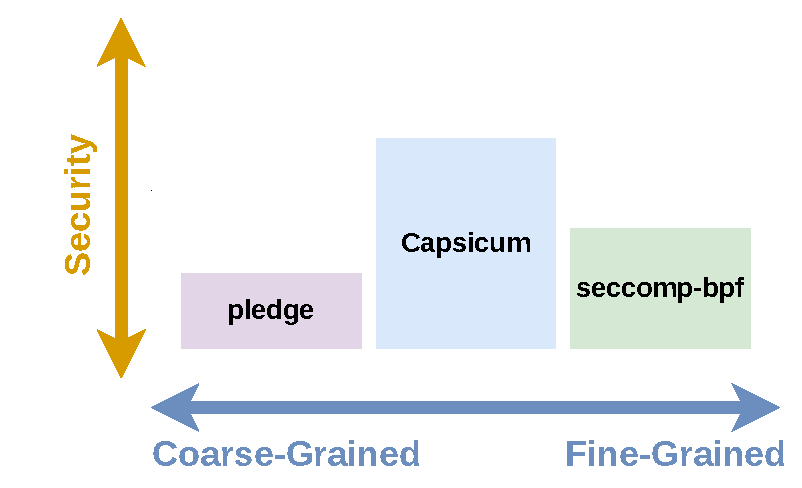
\includegraphics[width=0.8\linewidth]{figs/systemcall-interposition.pdf}
%    \caption{Security and granularity trade-offs of pledge,
%    Capsicum, and seccomp-bpf.}%
%    \label{fig:syscall_interposition}
%\end{figure}

In the original Linux seccomp implementation, processes use a special \texttt{seccomp(2)} system call to enter a secure computing state. By default, processes that have entered this state are restricted to performing \texttt{read(2)}, \texttt{write(2)}, \texttt{sigreturn(2)}, and \texttt{exit(2)} system calls.  Pragmatically, this means that a process could read and write on its open file descriptors, return from invoked signal handlers, and terminate itself. All violations of this policy would result in forced termination. In a 2012 RFC \cite{drewry2012_seccomp_bpf}, Drewry introduced an extension to seccomp, enabling the use of BPF programs for the defining filters on system call arguments. This extension, dubbed seccomp-bpf, enables creating fine-grained seccomp policies that filter on system call numbers and arguments, providing a high degree of control to applications that wish to sandbox themselves.

Despite the high degree of control that seccomp-bpf offers to applications, it has severe usability and security concerns, rendering it an unacceptable solution for ad-hoc confinement by end-users. Classic BPF \cite{mccanne1993_bpf} is a rather arcane bytecode language, and writing Classic BPF programs by hand is a task left only to expert users. Further, seccomp-bpf policy is easy to misconfigure, resulting in potential security violations; for instance, an attacker may entirely circumvent a policy that specifies restrictions on the \texttt{open(2)} system call but not \texttt{openat(2)}. Finally, despite userspace library efforts to abstract away the underlying BPF programs \cite{libseccomp}, seccomp-bpf remains accessible only to application developers with significant security expertise.

OpenBSD's pledge \cite{pledge} takes a more straightforward, coarser-grained approach to system call filtering than seccomp-bpf, instead grouping system calls into high-level semantically meaningful categories, such as \texttt{stdio} which includes \texttt{read(2)} and \texttt{write(2)}, for example \cite{anderson2017_comparison}. This coarse granularity and simplicity provide increased usability but come at the expense of expressiveness. There is no canonical way to distinguish subsets of system call groups or filter system calls by their arguments.  Despite its increased usability for developers, pledge still suffers from a lack of application transparency just as seccomp-bpf does, meaning that it is only suitable for application developers rather than end-users.

Unlike seccomp-bpf and pledge, which apply filtering rules to system calls directly, FreeBSD's Capsicum takes the approach of restricting access to global namespaces via a capability-based implementation \cite{watson2010_capsicum}. In Capsicum, a process enters \textit{capability mode}  using a special \texttt{cap\_enter} system call. Once in capability mode, access to global namespaces is restricted to the capabilities requested by the process. These capabilities are inherited across \texttt{fork(2)} and \texttt{execve(2)} calls.  Much like seccomp-bpf and pledge, however, Capsicum is \textit{not} application transparent and is designed for use by developers rather than end-users.

\paragraph*{Linux Security Modules}

The Linux Security Modules (LSM) API \cite{wright2002_lsm} provides an extensible security framework for the Linux kernel, allowing for the implementation of powerful kernelspace security mechanisms that can be chained together. LSM works by integrating a series of strategically placed \textit{security hooks} into kernelspace code. These hooks roughly correspond with boundaries for the modification of kernel objects. Multiple security implementations can hook into these LSM hooks and provide callbacks that generate audit logs and make policy decisions. \Cref{fig:lsm} depicts the LSM architecture in detail.

\begin{figure}[htb]
    \centering
    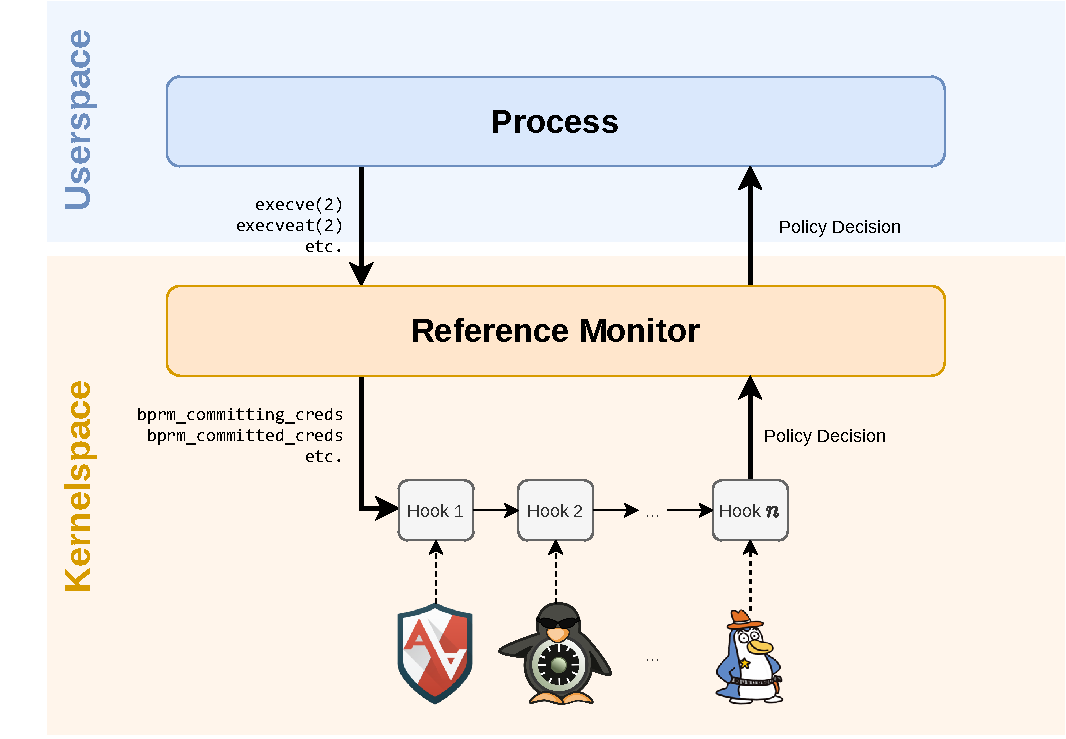
\includegraphics[width=0.8\linewidth]{figs/lsm.pdf}
    \caption{The LSM architecture. Note the many-to-many relation between access
    requests and hook invocations. Multiple LSM hooks may be chained together,
    incorporating policy from many security mechanisms. All hooks must agree to
    allow the access or it will be denied.}%
    \label{fig:lsm}
\end{figure}

The LSM API sits at a level of abstraction just above the system call API---a single LSM hook may cover multiple system calls, and a single system call may contain multiple such LSM hooks. For instance, the \texttt{execve(2)} and \texttt{execveat(2)} calls both result in a call to the \texttt{bprm\_committing\_creds} and  \texttt{bprm\_committed\_creds} hooks (among others).  This design provides a excellent level of abstraction compared to system-call-based approaches like seccomp-bpf \cite{seccomp_bpf, drewry2012_seccomp_bpf} in that a single LSM hook can cover all closely related security events (recall the issue of \texttt{open(2)} vs.~\texttt{openat(2)} in seccomp-bpf).

The Linux kernel contains several in-tree LSM-based security modules, which may be enabled by default on certain distributions.  Many such modules implement \textit{mandatory access control} (MAC) schemes, which enable fine-grained access control that can limit \textit{all users' privileges}---even the superuser. SELinux \cite{smalley2001_selinux} and AppArmor \cite{cowan2000_apparmor} are two such MAC LSMs, each with distinct policy semantics. I discuss each in turn.

SELinux \cite{smalley2001_selinux} was initially developed by the NSA as a Linux implementation of the Flask \cite{spencer1999_flask} security model.  Under SELinux, system subjects (e.g.~users or processes) and system objects (e.g.~files or network sockets) are assigned corresponding labels. Security policy is then written based on these labels, specifying the allowed access patterns between a particular object type and subject type. SELinux's policy language is famously arcane \cite{schreuders12_towards}. Despite multiple efforts to introduce automated policy generation \cite{audit2allow, macmillan07_madison, sniffen06_guided}, writing and auditing SELinux security policy remains a task for security experts rather than end-users. Further, due to the difficulty of writing and auditing the complex SELinux policy language, there is a natural tendency for human policy authors to err on the side of over-permission, violating the principle of least privilege.

AppArmor (originally called SubDomain) \cite{cowan2000_apparmor} is often touted as a more usable alternative to SELinux, although usability studies have shown that this claim merits scrutiny \cite{schreuders12_towards}. Rather than basing security policy on labelling system subjects and objects, AppArmor instead employs path-based enforcement. AppArmor defines policy in per-application profiles, which contain rules specifying what system objects the application can access. System objects are identified directly (for example, via pathnames, socket classes, or IP network addresses) rather than labelled.  AppArmor also supports the notion of \textit{changing hats}, through which a process may change its AppArmor profile under certain conditions specified in the policy.  Although AppArmor profiles are more conforming to standard Unix semantics than their SELinux counterparts, users who wish to write AppArmor policy still require a considerable amount of knowledge about operating system security \cite{schreuders12_towards}.

\subsection{Containers}
\label{subsection:containers}

Containers use OS-level virtualization and confinement mechanisms (c.f.~\Cref{subsection:low_level}) to provide a (semi-)isolated environment for the execution of processes \cite{sultan2019_container_security}. Since they run directly on the host operating system and share the underlying OS kernel, containers do not require a full guest operating system to implement virtualization. This technique has the advantage of offering a light-weight alternative to traditional hardware virtualization approaches using full virtual machines \cite{sultan2019_container_security}. Compared with containers, traditional approaches to virtualization involve hypervisors, which virtualize and provide access to the underlying hardware, either running on top of a host operating system or directly on top of the hardware itself. Full virtual machines run on top of these hypervisors, each running a guest operating system with a full userland and kernel. Full virtualization provides stronger isolation guarantees than containers but involves significantly more overhead imposed by the guest operating system \cite{sultan2019_container_security}. \Cref{fig:virt} depicts an overview of the architectural differences between containers and full hardware virtualization solutions (i.e.~virtual machines running on top of hypervisors).

\begin{figure}[htb]
  \centering
  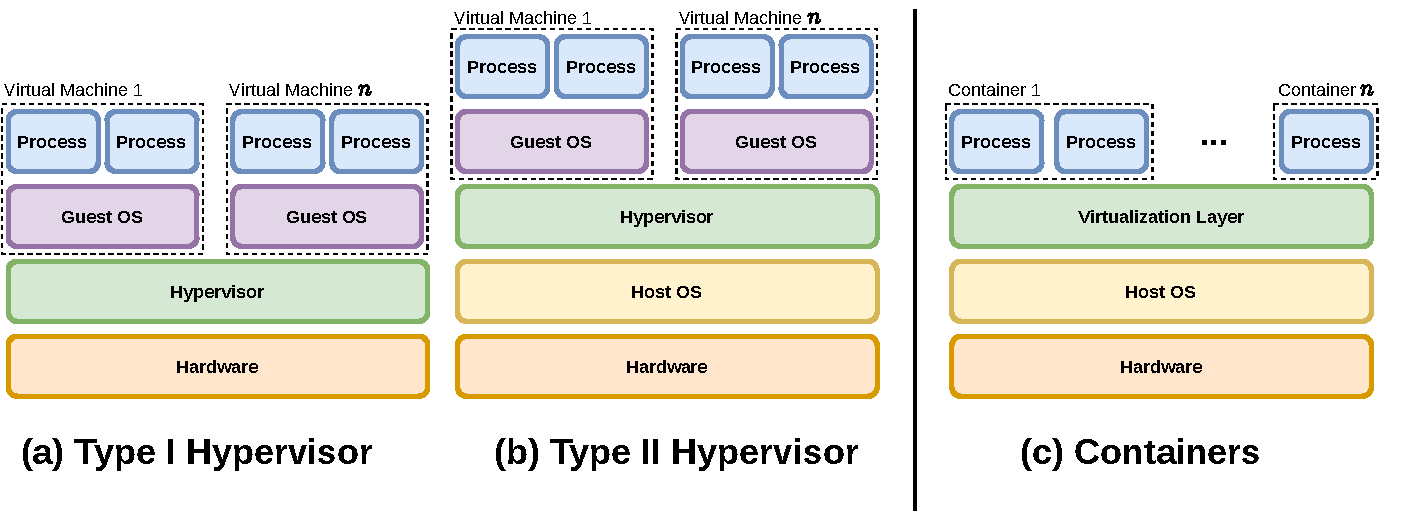
\includegraphics[width=1\linewidth]{figs/virtualization.pdf}
  \caption{
    Virtual machine and container architectures. Type I hypervisors \textbf{(a)} virtualize and control the underlying hardware directly, but require full guest operating systems on top of the virtualization layer. Type II hypervisors \textbf{(b)} run on top of a host operating system but still require full guest operating systems above the virtualization layer. Containers \textbf{(c)} achieve virtualization using a thin layer provided by the host operating system itself. They share the underlying operating system kernel and resources, requiring no guest operating system \cite{sultan2019_container_security}.
  }%
  \label{fig:virt}
\end{figure}

Since containers must share the host operating system kernel and related resources, it is essential to consider how best to isolate them from one another. Therefore, a container management system generally seeks to achieve the following security-related goals\footnote{Dependency management is another goal of container management systems like Docker \cite{docker}, Kubernetes \cite{kubernetes}, and OpenShift \cite{openshift}, but it is out of scope for his paper.}:
\begin{enumerate}[label=\bfseries CG\arabic*., ref=CG\arabic*, labelindent=1em]
  \item \textsc{Virtualization.}
    Virtualization aims to provide each container with a \textit{virtual view} of system resources. Containers generally achieve virtualization using a combination of Linux namespaces, cgroups, and filesystem mounts. Namespaces provide a private view of enumerable resources (i.e.~a virtual mapping of IDs to resources). Such enumerable resources include process IDs, user and group IDs, mountpoints, and the network interfaces. Cgroups similarly provide a virtual view of \textit{quantifiable resources} (i.e.~how much of a given resource is available). Such quantifiable resources include the CPU, persistent storage, memory, and I/O bandwidth. Filesystem mounts, combined with mount namespaces, provide a virtual view of visible files.

    Although full virtualization may be desirable in the ideal case, containers often only implement partial virtualization \cite{sultan2019_container_security,xin2018_container_security} due to various factors. Pragmatically, it is often beneficial for containers to have a shared view of specific system resources, depending on the use case. For instance, two containers might share a copy of the same shared library or require access to a shared IPC namespace to enable communication. In practice, containers often leverage layered filesystems such as overlayfs \cite{edge2010_overlayfs} to deduplicate files across containers and the host system. Partial virtualization can enable lighter-weight containers and easier communication between two containers to satisfy composability \cite{sultan2019_container_security}.

  \item \textsc{Least-Privilege.}
    For a container to be considered secure, it must enforce least-privilege on its processes \cite{sultan2019_container_security}. This requirement makes practical sense, given that a container runs directly on the host system and must share the underlying OS kernel and resources with both other containers and the host system itself. Without least-privilege, a process running in a container has virtually the same access rights as an unconfined process. When the container itself is running with privileged access to the system (as is often the case \cite{sultan2019_container_security,xin2018_container_security}), this may even result in an \textit{escalation of privilege} compared to the scenario where the process runs directly on the host. For these reasons, it is neither practical nor advisable to rely on weak virtualization guarantees to protect the host system with no means of enforcing least-privilege \cite{sultan2019_container_security}.

    A least-privilege implementation for containers typically involves a combination of multiple enforcement mechanisms, including Unix DAC, seccomp-based system call filtering, dropped POSIX capabilities, and mandatory access control mechanisms (using one of the Linux MAC LSMs) \cite{sultan2019_container_security,xin2018_container_security,docker}. This complexity can lead to usability and auditability concerns, as a simple policy language must compile down to multiple complex enforcement mechanisms that need to work cooperatively \cite{findlay2020_bpfbox}.

    Despite its evident importance for container security, existing container management solutions generally treat least-privilege as a secondary goal \cite{sultan2019_container_security}. Docker attempts to provide sensible security defaults for containers. Still, these defaults may be easily overridden and often rely on extra kernel security features such as the AppArmor LSM \cite{docker}. When AppArmor is not available, Docker falls back to relying exclusively on its default seccomp policy and dropped capabilities. Security defaults for containers also often do not adhere to the principle of least privilege. For instance, Docker provides containers with 15 Linux capabilities by default, including \texttt{CAP\_DAC\_OVERRIDE}, which allows a container to override all discretionary access control checks \cite{sultan2019_container_security,docker}.

  \item \label{item:composability} \textsc{Composability.}
    Increasingly, containers are being used to implement composable microservices \cite{sultan2019_container_security}. For instance, Kubernetes \cite{kubernetes} allows the user to group containers into \textit{pods}, allowing them to communicate with each other in pre-defined ways. For composability, a container needs the ability to communicate with another container without sacrificing virtualization or least-privilege. In practice, containers achieve such composability by defining specific inter-container exceptions to virtualization and least-privilege policy \cite{sultan2019_container_security}. Naturally, these exceptions can increase the risk of an insecure configuration, and the user must carefully manage them to avoid overprivilege.
\end{enumerate}

%\todo{Discuss prominent examples: Docker, Kubernetes}
%\todo{Discuss containerized package management: Snap, FlatPak}

\subsection{Classic and Extended BPF}

The original Berkeley Packet Filter (BPF) \cite{mccanne1993_bpf}, hereafter referred to as Classic BPF, was a packet filtering mechanism implemented initially for BSD Unix. McCanne and Jacobson created Classic BPF as a light-weight replacement for traditional packet filtering mechanisms, which relied on frequent context switches between userspace and kernelspace while making filtering decisions. Instead, Classic BPF implemented a simple register-based virtual machine language and efficient buffer data structures to minimize the required context switches. As an efficient packet filtering mechanism, Classic BPF quickly gained traction in the *NIX community and was subsequently ported to various open-source Unix and Unix-like operating systems, most notably Linux \cite{linux_bpf}, OpenBSD \cite{openbsd_bpf}, and FreeBSD \cite{freebsd_bpf}.

The Linux kernel development community eventually realized that the BPF engine could be applied to more than just packet filtering. The 2012 introduction of seccomp-bpf \cite{drewry2012_seccomp_bpf,seccomp_bpf} enabled Classic BPF programs to be written and applied to make system call filtering decisions for userspace applications. This extension to seccomp transformed it into a powerful (yet notoriously difficult-to-use \cite{anderson2017_comparison}) mechanism for making security decisions about system calls in a confined process.

In 2014, Starovoitov and Borkmann merged a complete rewrite of the Linux BPF engine, dubbed Extended BPF (eBPF), into the mainline kernel \cite{starovoitov2014_ebpf}. eBPF expands on the original BPF specification by introducing:
\begin{itemize}
  \item An extended instruction set;
  \item 11 registers (10 of which are general-purpose);
  \item Access to allow-listed kernel helpers;
  \item Just-in-time (JIT) compilation to native instruction sets;
  \item A program safety verifier;
  \item A large collection of specialized data structures; and
  \item New program types which can be attached to a variety of system events in both userspace and kernelspace.
\end{itemize}
These extensions to the Classic BPF engine effectively turn eBPF into a general-purpose execution engine in the kernel with powerful system introspection and kernel extension capabilities. eBPF programs execute in the kernel with supervisor privileges but are limited by a restricted execution context and pre-checked for safety by an in-kernel verification engine. In particular, eBPF programs are limited to a 512-byte stack, cannot access unbounded memory regions, must not have back-edges in their control flow, and must provably terminate \cite{gregg2019_bpf}. As a consequence of these restrictions, eBPF programs are not Turing-complete. Where necessary, an eBPF program can make calls to a set of allow-listed kernel helpers to obtain additional functionality, such as access to external memory regions and various kernel facilities such as signalling or random number generation \cite{gregg2019_bpf}.

\begin{figure}[htb]
  \centering
  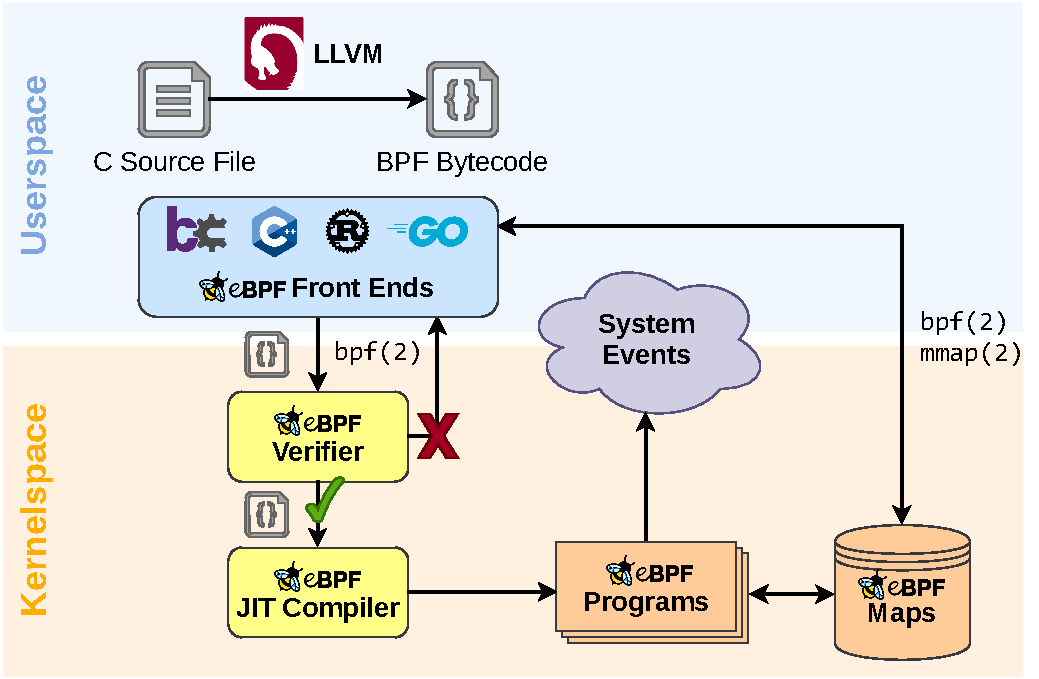
\includegraphics[width=0.8\linewidth]{figs/ebpf.pdf}
  \caption{
    eBPF mechanisms in the kernel. Userspace front-ends compile C source code into eBPF bytecode using the LLVM toolchain and load it into the kernel with the \texttt{bpf(2)} system call. The in-kernel verifier either accepts or rejects the program based on its adherence to safety invariants. Accepted programs are attached to system events across the userspace and kernelspace boundary where they are just-in-time compiled to the native instruction set. Programs can store and fetch data using data structures called \enquote{eBPF maps}, which can also be accessed directly from userspace.
  }%
  \label{fig:ebpf}
\end{figure}

A privileged userspace process may load an eBPF program into the kernel using Linux's \texttt{bpf(2)} system call. While it is possible to write eBPF bytecode by hand \cite{gregg2019_bpf}, several front-ends exist for compiling eBPF bytecode from a restricted subset of the C programming language\footnote{In principle, this language need not be C. For instance, a framework exists for writing eBPF programs in pure Rust \cite{redbpf}. However, C is a popular choice since it is tightly coupled with the underlying implementation of the kernel.}, including bcc \cite{bcc} and libbpf \cite{libbpf}. These front-ends typically use the LLVM \cite{llvm_bpf} compiler toolchain to produce BPF bytecode. When the kernel receives a request to load an eBPF program, it first checks the bytecode to ensure that it conforms to the safety invariants outlined above. If the verifier accepts the program, it may then be attached to one or more system events. When an event fires, the eBPF program is executed via just-in-time compilation to the native instruction set. eBPF programs can store data in several specialized in-kernel data structures, made accessible to userspace via the \texttt{bpf(2)} system call or a direct memory mapping. \Cref{fig:ebpf} depicts this process in detail.



\section{Motivation}
\label{sec:motivation}

\subsection{Threat Model}%
\label{sub:threat_model}

Sultan \etal~\cite{sultan2019_container_security} propose four broad categories of container-related threats. \Cref{fig:threat_model} presents an overview of each category. An application running within a container might attack the container itself, attempting to escape confinement or interfere with the execution of co-located applications running within the same container. Inter-container threats are similarly possible, wherein one container attempts to interfere with or take over another. Since containers share the underlying host operating system, it is also possible for a container to directly attack the host, either by escaping confinement altogether or by launching denial of service or resource consumption attacks. Finally, a malicious or semi-honest host system may attack containers running within it. Researchers have generally recognized that mitigating this fourth category of attack requires the use of hardware security mechanisms \cite{sultan2019_container_security} \todo{cite others} such as trusted execution environments or trusted platform modules. Such host-to-container attacks are, therefore, out of scope for this paper.

\begin{figure}[htpb]
  \centering
  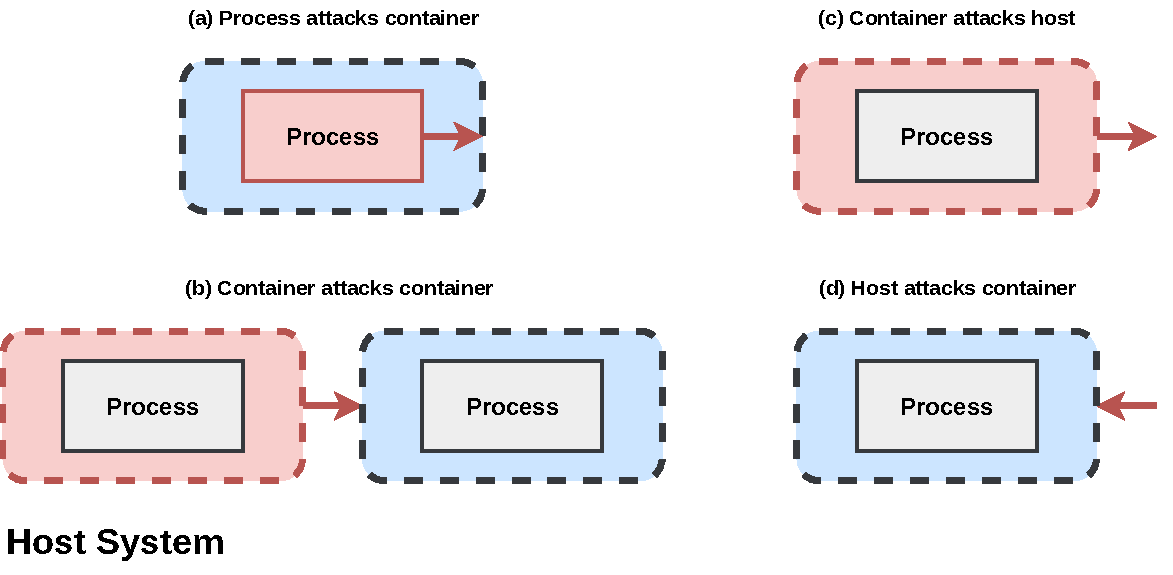
\includegraphics[width=0.8\linewidth]{figs/threat-model.pdf}
  \caption{
    Four categories of container-related attacks \cite{sultan2019_container_security}. \textbf{(a)} A process running within a container attacks the container itself. \textbf{(b)} One container attacks another container. \textbf{(c)} A container attacks the host system. \textbf{(d)} The host system attacks the container. This fourth category of attack is out of scope for this paper.
  }%
  \label{fig:threat_model}
\end{figure}

In this threat model we consider three broad classes of attack vector, comprised of the containers and the applications that run within them. These attack vectors are described in turn below.
\begin{enumerate}[label=\bfseries AV\arabic*., ref=AV\arabic*, labelindent=1em]
  \item \textsc{Malicious Applications.}
    A malicious application is designed with express malicious intent. Malicious software may actively attempt to subvert other applications, other containers, or the host system itself. This subversion could include privilege escalation attacks on the host system, denial of service attacks on other containers or the host, or the installation of backdoors. A sophisticated attacker could even abuse a malicious application to install a rootkit \cite{beegle2007_rootkit} in the container, on the host system, or in the host's firmware, stealthily gaining permanent and possibly overprivileged access.
  \item \textsc{Semi-Honest Applications.}
    In contrast with malicious applications, semi-honest applications are not necessarily expressly designed with malicious intent and might even be cooperative with other applications or containers. However, the semi-honest application can passively participate in unwanted activity, such as surveillance or consumption of the host's resources.
  \item \textsc{Vulnerable Applications.}
    Vulnerable applications running inside containers may become compromised by attackers, often with the goal of using these applications to orchestrate a more sophisticated attack on other applications running within the same container, other containers, or the host system itself \cite{sultan2019_container_security}. Common vulnerabilities here include code execution vulnerabilities on untrusted input, memory corruption bugs, and privilege escalation vulnerabilities in a container's configuration. Exploitation of kernel-level vulnerabilities are also a concern here, as an attacker can potentially abuse a legitimate application to target vulnerable code paths in the kernel \cite{xin2018_container_security}.
\end{enumerate}

Since containers are often co-located in large-scale, multi-tenant systems such as the cloud \cite{sultan2019_container_security}, the potential for exploitation or abuse by foreign threat actors is exacerbated. Thus, it is imperative that container management systems enforce least-privilege on containers to prevent such exploitation from negatively impacting the rest of the system.

\subsection{The Quest for Secure Containers}%
\label{sub:secure_containers}

\subsection{Why an eBPF Implementation?}%
\label{sub:why_ebpf}

\todo{
\begin{itemize}
  \item Can be dynamically loaded without rebooting the kernel
  \item Guaranteed safety
  \item Can be used in production without downtime
  \item Container-specific LSM $\rightarrow$ Only apply policy to a given container
  \item Dynamically instrument non-lsm functions in the kernel, such as \texttt{commit\_creds}, this allows us to prevent kernel privilege escalation attacks like the ones described in Xin \etal~\cite{xin2018_container_security}
\end{itemize}
}


\section{\bpfcontain{} Design and Implementation}
\label{sec:design}

\todo{Introduce \bpfcontain{} and talk about how it attempts to solve container security}

\subsection{Design Goals}

Five specific goals informed the design of \bpfcontain{}'s policy language and
enforcement mechanism, enumerated below as Design Goals \ref{d:1} to \ref{d:5}.
%Note that there is a natural interplay between some of these design goals, while
%others are typically perceived as being in contention (specifically usability
%and security). In cases of conflict, it is essential to strike a careful balance
%between each property.

\begin{enumerate}[label=\bfseries D\arabic*., ref=D\arabic*, labelindent=1em]
  \item \label{d:1} \textsc{Usability.}
    \bpfcontain{} should not impose unnecessary usability barriers on end-users.  Its policy language should be easy to understand and semantically meaningful to users without requiring significant security knowledge. To accomplish this goal, \bpfcontain{} takes some inspiration from other high-level policy languages for containerized applications, such as those used in Snapcraft \cite{snap}.

  \item \label{d:2} \textsc{Configurability.}
    It should be easy for an end-user to reconfigure policy to match their specific use case without worrying about the operating system's underlying details or the policy enforcement mechanism. It should be possible to use \bpfcontain{} to restrict specific unwanted behaviour in a given application without needing to write a rigorous security policy from scratch.

  \item \label{d:3} \textsc{Transparency.}
    Confining an application using \bpfcontain{} should not require modifying the application's source code or running the application using a privileged SUID (Set User ID root) binary. \bpfcontain{} should be entirely agnostic to the rest of the system and should not interfere with its regular use.

  \item \label{d:4} \textsc{Adoptability.}
    \bpfcontain{} should be adoptable across a wide variety of system configurations and should not negatively impact the running system. It should be possible to deploy \bpfcontain{} in a production environment without impacting system stability and robustness or exposing the system to new security vulnerabilities. \bpfcontain{} relies on the underlying properties of its eBPF implementation to achieve its adoptability guarantees.

  \item \label{d:5} \textsc{Security.}
    \bpfcontain{} should be built from the ground up with security in mind. In particular, security should not be an opt-in feature, and \bpfcontain{} should adhere to the principle of least privilege \cite{saltzer1975_protection} by default. It should be easy to tune a \bpfcontain{} policy to respond to new threats.
\end{enumerate}

\subsection{Architectural Overview}
\label{sub:architecture}

\bpfcontain{} consists of both userspace and kernelspace components, which interact co-operatively to implement its policy enforcement mechanism. Roughly, its architecture (depicted in \Cref{fig:architecture}) can be broken down into the following four components:
\begin{enumerate}[label=\bfseries C\arabic*., ref=C\arabic*, labelindent=1em]
  \item \label{c:1}
    A privileged daemon, responsible for loading and managing the lifecycle of eBPF programs and maps and logging security events to userspace.

  \item \label{c:2}
    A small shared library and unprivileged wrapper application used to initiate confinement.

  \item \label{c:3}
  A set of eBPF programs, running in kernelspace. These programs are attached to LSM hooks in the kernel as well as the shared library in \ref{c:2}.

  \item \label{c:4}
  A set of eBPF maps, special data structures which allow bidirectional communication between userspace and kernelspace. These maps are used to track the state of running containers and store the active security policy for each container.
\end{enumerate}

\begin{figure}[htb]
  \centering
  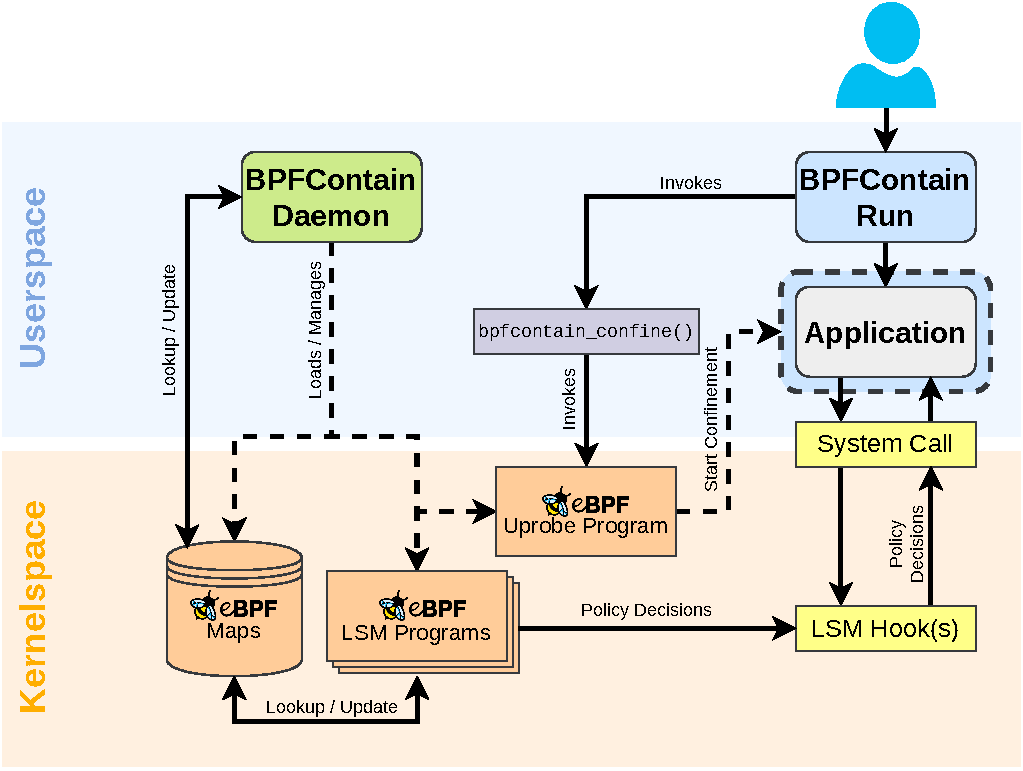
\includegraphics[width=0.8\linewidth]{figs/architecture.pdf}
  \caption{
    A diagram of \bpfcontain{}'s architecture. The privileged daemon (green) is responsible for loading the necessary eBPF maps and programs (orange) into the kernel and managing their lifecycle. The user starts a container by executing an unprivileged wrapper application (blue), which invokes the \texttt{bpfcontain\_confine} library call (purple), trapping to a special eBPF program that associates the process group with the right policy.  When the confined application (grey) makes a system call to request access to a sensitive resource, the kernel invokes one or more LSM hooks (yellow), which trap to corresponding eBPF LSM programs that make the correct policy decision.
  }%
  \label{fig:architecture}
\end{figure}

In userspace, \bpfcontain{} is implemented as a privileged daemon based on the bcc \cite{bcc} eBPF framework for Python. The daemon is responsible for loading \bpfcontain{}'s eBPF programs and maps and logging security events to userspace, such as policy violations.  When it first starts, the daemon invokes a series of \texttt{bpf(2)} system calls to load its eBPF programs and maps into the kernel. After loading all eBPF programs and maps, the daemon then parses, translates, and loads each per-container policy file into several eBPF maps.

For the bulk of its policy enforcement \bpfcontain{} leverages the KRSI (kernel runtime security instrumentation) patch merged by KP Singh~\cite{singh2019_krsi,corbet2019_krsi} into the Linux 5.7 kernel. This patch enables eBPF programs to be attached to LSM hooks at runtime, making policy decisions and log security events.  These programs work cooperatively with each other and with any other LSMs running on the system to come to a policy decision. When an event fires, the LSM programs query policy from policy maps to come to a decision. This dynamic runtime policy enforcement is at the core of \bpfcontain{}'s flexible container security approach.

\subsection{\bpfcontain{} Policy}
\label{sub:policy}

\bpfcontain{} policy consists of simple manifests written in YAML \cite{yaml}, a human-readable data serialization language based on key-value pairs.  Each \bpfcontain{} container is associated with a manifest, which itself consists of a few lines of metadata followed by a set of \textit{rights} and \textit{restrictions}.  A \textit{right} specifies access that should be granted to a container, while a \textit{restriction} is used revoke access. While rights and restrictions may be combined at various granularities, a restriction always overrides a right of the same or coarser granularity. For instance, a right to access the root filesystem would be overridden by a restriction on the user's home directory. In practice, this allows the construction of nuanced policies that specify coarse-grained access with finer-grained exceptions.  \Cref{tab:accesses} describes the various access labels that can be used in \bpfcontain{} policy.

{
\small
\begin{longtable}[c]{llp{25em}}
  \caption{
    Access labels for \bpfcontain{} policy along with their parameters and descriptions. Square brackets denote an optional parameter.
  }
  \label{tab:accesses}\\
  \toprule
  Resource              & Parameters          & Description \\
  \midrule
  \endfirsthead
  \texttt{filesystem} & Mountpoint, [Access] &
    Grants or revokes access at the granularity of a filesystem mountpoint. Access defaults to read, write, append, chdir, create, and setattr, unless otherwise specified. An optional \texttt{readonly} flag grants read and chdir access. An optional \texttt{appendonly} flag grants read, append, setattr, create, and chdir access. \\
  \texttt{file}       & Pathname, Access  &
    Grants or revokes access at the granularity of individual files. Access must be specified as a string of access flags (see \Cref{tab:fs_policy}). \\
  \midrule
  \texttt{net-bind} &  &
    Grants or revokes access to the \texttt{CAP\_NET\_BIND\_SERVICE} POSIX capability, allowing the container to bind to privileged ports. \\
  \texttt{net-raw} &  &
    Grants or revokes access to the \texttt{CAP\_NET\_RAW} POSIX capability, allowing the container to use raw sockets. \\
  \texttt{net-broadcast} &  &
    Grants or revokes access to the \texttt{CAP\_NET\_BROADCAST} POSIX capability, allowing the container to broadcast and listen to multicast network traffic. \\
  \texttt{dac-override} &  &
    Grants or revokes access to the \texttt{CAP\_DAC\_OVERRIDE} POSIX capability, allowing the container to override discretionary access controls. \\
  \midrule
  \texttt{network}    & [Family], [Access] &
    Grants or revokes access to network communications. A specific address family and access pattern may optionally be specified. \\
  \texttt{ipc}        & Container           &
    Grants or revokes access to communicate with processes in \textit{another} \bpfcontain{} container. This covers all supported System V IPC categories as well as Unix sockets and signals. Both containers must mutually declare IPC access. \\
  \midrule
  \texttt{tty}        & [Access]            &
    Grants or revokes access to terminal devices. \\
  \texttt{pts}        & [Access]            &
    Grants or revokes access to pseudo-terminal devices. \\
  \texttt{video}      & [Access]            &
    Grants or revokes access to video devices. \\
  \texttt{sound}      & [Access]            &
    Grants or revokes access to sound devices. \\
  \texttt{graphics}   & [Access]            &
    Grants or revokes access to graphics devices. \\
  \texttt{random}   & [Access]            &
    Grants or revokes access to random and urandom devices. \\
  \multicolumn{3}{c}{...} \\
  \bottomrule
\end{longtable}
}

\bpfcontain{} provides three policy granularities for file access: filesystem rules, file rules, and device rules. A filesystem rule grants access to an entire filesystem, specified by providing the pathname of its mountpoint. For instance, a policy would specify access to the root filesystem with \texttt{filesystem /} and procfs with \texttt{filesystem /proc}. File rules specify access at the granularity of individual files and directories. Finally, coarse-grained device rules such as tty, pts, video, and sound specify access at the granularity of common character and block devices. Each file access rule supports 13 specific access categories (outlined in \Cref{tab:fs_policy}) which may be combined as necessary. Filesystem rules also support two coarse-grained access flags, \texttt{readonly} and \texttt{appendonly}, which act as shortcuts for commonly-used access flags for filesystems.

{
\small
\begin{longtable}[c]{llp{25em}}
  \caption{
    Access categories for filesystem and file policy.
  }
  \label{tab:fs_policy}\\
  \toprule
  Access             & Flag       & Description \\
  \midrule
  \endfirsthead
  Read               & \texttt{r} & The container may read the file. This does not apply to directories. \\
  Write              & \texttt{w} & The container may write to the file. This does not apply to directories. \\
  Execute            & \texttt{x} & The container may execute the file (via execve). This does not apply to directories. \\
  Append             & \texttt{a} & The container may append to the file (without overwriting existing contents). This does not apply to directories.\\
  Create             & \texttt{c} & The container may create new files in the directory. \\
  Rename             & \texttt{n} & The container may rename the file or directory. \\
  Delete             & \texttt{d} & The container may delete the file or directory. \\
  Change Directory   & \texttt{t} & The container may change directory into this directory. \\
  Set Attribute      & \texttt{s} & The container may set attributes on this file or directory. \\
  Change Permissions & \texttt{p} & The container may change permissions on the file or directory. \\
  Change Owner       & \texttt{o} & The container may change the owner of the file or directory \\
  Link               & \texttt{l} & The container may create a hard link to the corresponding inode. \\
  Execute Mapped     & \texttt{m} & The container may map the file into memory for execution (other \texttt{mmap} operations are governed normally by read, write, and append access). This allows policy to distinguish shared libraries from executables. \\
  \bottomrule
\end{longtable}
}

\bpfcontain{} defines four capability rules which are used to specify exceptions to its default-deny policy on POSIX capabilities. The \texttt{netbind} rule grants the ability to bind to privileged ports, the \texttt{netraw} rule grants the ability to use raw sockets, and the \texttt{netbroadcast} rule grants the ability to broadcast and listen to multicast network traffic. The \texttt{dac-override} rule grants the ability to override discretionary access controls on files. All other POSIX capabilities are implicitly denied and may not be overridden. Note that these capability rules may not be used to grant overpermission to a container---the underlying process must already have the actual capability to use it.

Network policy in \bpfcontain{} enforces at the socket level, across various granularities. The most basic network policy consists of a single rule \texttt{network} which grants coarse-grained access to the entire networking stack. A specific address family and level of access may also be specified for finer-grained policy. Network policy is closely related to IPC policy, which grants or revokes permission to perform interprocess communication between containers. Support IPC mechanisms include System V IPC, signals, and Unix sockets (which must also be declared under network policy). For inter-container IPC to be valid, \textit{both} containers must mutually declare IPC access to each other. In other words, if container $A$ wishes to perform IPC with container $B$, container $A$ must list an \lstinline[language=yaml]{ipc: B} right and container $B$ must also list an \lstinline[language=yaml]{ipc: A} right.

%\todo{Maybe cover some policy examples}

\subsection{Launching a \bpfcontain{} Container}
\label{sub:launching}

To allow processes to request that they be placed into a container, \bpfcontain{} attaches a specialized eBPF program type called a \texttt{uprobe} (userspace probe) to a userspace library call, \texttt{bpfcontain\_confine}.  This function is a stub, whose only purpose is to trap to the uprobe---if it fails to trap the corresponding eBPF program (for example if \bpfcontain{} has not yet loaded its eBPF programs into the kernel), the function returns \texttt{-EAGAIN} to indicate that the caller should repeat the request. Attaching a \texttt{uprobe} to a library call in this way is a common eBPF design pattern, which effectively allows eBPF programs to make almost arbitrary extensions to the kernel's API.

When \texttt{bpfcontain\_confine} traps to its corresponding uprobe, the uprobe queries the current PID and associates that PID with a corresponding container ID. This container parameterizes \bpfcontain{}'s policy maps, allowing it to query the given container's correct policy. Subsequent forks associate newly created processes with the parent's container ID, assuring that the entire process subtree belongs to the same container. Once a process has been associated with a specific container ID, this association persists until the process exits, preventing the \texttt{bpfcontain\_confine} call from being abused to transition to another container profile.

From the user's perspective, running a \bpfcontain{} container is as simple as invoking the \texttt{bpfcontain run -n <name>} command. This command is a thin wrapper around the \texttt{bpfcontain\_confine} library call discussed above. Its only purpose is to invoke this library call, check for a successful invocation (using its return value), and then execute the command defined in the corresponding container manifest. See \Cref{fig:launch} for an overview of this process.

\begin{figure}[htb]
  \centering
  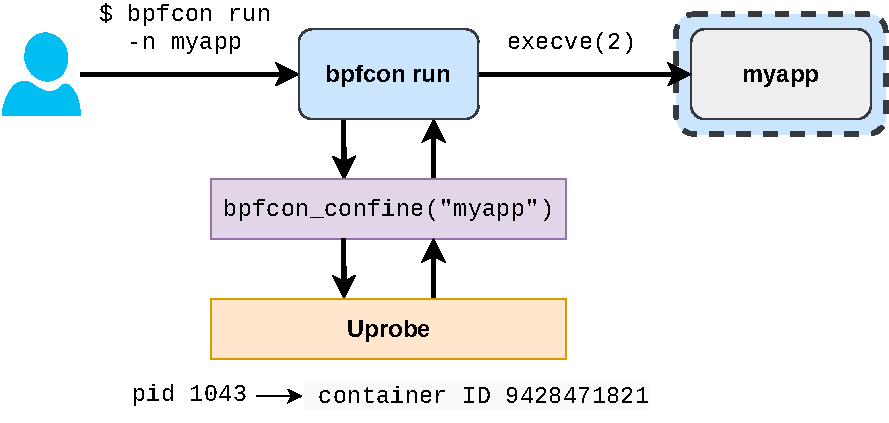
\includegraphics[width=0.6\linewidth]{figs/launch.pdf}
  \caption{Launching a \bpfcontain{} container.}%
  \label{fig:launch}
\end{figure}

\todo{Not sure if I really want to say this or not}
An important feature of \bpfcontain{} is that the \lstinline[language=c]|bpfcontain_confine| library call requires no additional operating system privileges to start confinement.  This notion of unprivileged confinement is a unique advantage over other container implementations in Linux.  Somewhat counter-intuitively, traditional container implementations often rely on binaries with escalated privileges (e.g.~setuid root) to set up proper confinement.  Failure to correctly drop these elevated privileges may result in \textit{escalation of privilege} in the host system, particularly if the confined process manages to escape the container.  By obviating this need for elevated privileges, \bpfcontain{} conforms with the principle of least privilege and improves its overall security.

As a side effect of \bpfcontain{}'s design, it is also possible for a generic application to invoke the \lstinline[language=c]|bpfcontain_confine| library call directly, eliminating the need to start the target application using the \texttt{bpfcontain run} wrapper. This notion of self-confinement enables application developers and package maintainers to ship \bpfcontain{} policy with their software and enforce it transparently to the end-user. Since \bpfcontain{} policy is designed to be readable and modifiable by end-users, a security policy shipped with an application could optionally be tuned by the user according to their specific needs.

\subsection{Policy Enforcement Mechanism}
\label{sub:enforcement}

%\bpfcontain{} only enforces security policy on processes which are currently
%associated with a container. The list of processes associated with a container
%is tracked using an eBPF map, which is updated whenever a process invokes the
%\texttt{bpfcontain\_confine} library call (assuming it is not already in
%a container), and whenever a process that is currently in a container forks
%itself. Once a process has been associated with a container, it remains
%associated with that container until it terminates.

Security policy in \bpfcontain{} falls into two categories: \textit{implicit} and \textit{explicit}. Explicit policy is per-container policy defined by the end-user in the container's manifest (see \Cref{sub:policy}). On the other hand, implicit policy comprises the set of sensible defaults which are applied and enforced for every container, regardless of its configuration. The vast majority of implicit \bpfcontain{} policy consists of behavioural restrictions, which prohibit a container from performing a set of dangerous actions which could be used to escape confinement, attack other containers, or negatively impact the host system. Conversely, other implicit policy grants a minimal set of rights to a container, including the ability to interact with its own procfs entries, communicate with other processes running in the same container, and access newly created files by processes within the container (e.g.~temporary files). \Cref{tab:implicit} describes each implicit policy category in \bpfcontain{}.

\begingroup
\small
\begin{longtable}[c]{llp{25em}}
  \caption{
    Implicit policy in \bpfcontain{}, which is enforced regardless of a container's manifest. Implicit restrictions generally correspond with resources which a well-behaved container should never need. Implicit rights permit certain sane behaviours, such as interprocess communication between processes \textit{within} a container. These rights effectively constitute exceptions to ordinary enforcement. Note that implicit rights may still be overridden by an explicit restriction specified in the container's manifest. A third category, implicit death, refers to accesses that cause \bpfcontain{} to send an uncatchable SIGKILL to the process.
  }
  \label{tab:implicit}\\
  \toprule
  Policy & Kind & Description \\
  \midrule
  \endfirsthead
  BPF & Restriction &
    A container is disallowed from making \textit{any} \texttt{bpf(2)} system calls. This restriction prevents a container from loading, unloading, and accessing any eBPF programs and maps, including those which belong to \bpfcontain{} itself. \\
  Ptrace & Restriction &
    A container may not use \texttt{ptrace(2)} to trace or control processes. \\
  Kernel Lockdown & Restriction &
    A container is subject to full Kernel Lockdown \cite{lockdown} restrictions, disabling all operations that could be used for arbitrary code execution in the kernel. \\
  Kernel Modules & Restriction &
    A container may not load any modules into the kernel. \\
  Kexec & Restriction &
    A container may not use \texttt{kexec}-family system calls to load new kernels. \\
  Shutdown & Restriction &
    A container may not shut down or reboot the system. \\
  Key Management & Restriction &
    A container may not interface with the kernel's key management mechanisms. \\
  Quotactl & Restriction &
    A container cannot use the \texttt{quotactl(2)} system call to bypass restrictions on resource consumption. \\
  Rlimit & Restriction &
    A container cannot use the \texttt{getrlimit(2)}, \texttt{setrlimit(2)}, or \texttt{prlimit(2)} system calls to get or set resource limits. \\
  Scheduler & Restriction &
    A container cannot inspect or modify process scheduling or I/O scheduling priority. \\
  Mount & Restriction &
    A container cannot mount, remount, unmount filesystems or move filesystem mounts. \\
  Pivot Root & Restriction &
    A container cannot pivot the root directory of a filesystem. \\
  Syslog & Restriction &
    A container cannot use the \texttt{syslog(2)} system call to access the kernel logs. \\
  Set Time & Restriction &
    A container cannot use the \texttt{settime(2)} system call to change the system time. \\
  \midrule
  Privilege Escalation & Death &
    To prevent kernel privilege escalation exploits which typically rely on forcing the execution of \texttt{commit\_creds} \cite{xin2018_container_security}, \bpfcontain{} will outright kill a contained process that invokes this function (outside of the execve code path) to try to escalate its privileges. \\
  \midrule
  IPC & Right &
    A process can always perform interprocess communication with another process within the same container. \\
  Procfs & Right &
    A process is granted full access to its own procfs entries, as well as those belonging to other processes within the same container. \\
  New Files & Right &
    A container is granted full access to any new files or directories that it creates. \\
  \bottomrule
\end{longtable}
\endgroup

Following the principle of least privilege \cite{saltzer1975_protection}, \bpfcontain{} implements strict default-deny enforcement. The user may optionally change this behaviour and elect to enforce a default-allow policy instead, by setting \lstinline[language=yaml]|default: allow| in the manifest. A default-allow policy enables the easy restriction of specific unwanted behaviour in a given program, without worrying about the details of constructing a rigorous security policy.  Unless a container has been marked as default-allow, all access requests which are not covered under the implicit or explicit policies for a container are denied by default, and the access request is logged to userspace by the \bpfcontain{} daemon. %[ <-- workaround for annoying VimTex syntax highlighting bug

\subsubsection{LSM Probes and Maps}

At runtime, \bpfcontain{} stores representations of explicit policy rules using several eBPF maps. In particular, it uses two maps for each major policy category, one to store allowed access patterns and another to store denied access patterns. \bpfcontain{} keys each policy map using a composite key comprised of a unique container ID combined with another unique identifier for the given resource. For instance, a filesystem policy key consists of the container ID and a unique filesystem device ID provided by the kernel. File policy keys are similar, but with the addition of an inode number to identify a specific file. Each key in a policy map maps to a vector describing the allowed or denied access pattern.

\bpfcontain{} also maintains a few other eBPF maps in addition to its policy maps, used to track the state of running processes, the containers they belong to, and other aspects of the running system, such as which procfs inodes belong to which containers. When \bpfcontain{} makes a policy decision, it considers the policy associated with the current container and the current state stored in these maps. For explicit policy, \bpfcontain{} compares the requested access vector with the values stored in its policy maps. For access to be allowed, the entire access vector must be a subset of the value stored in the \enquote{allow} policy map. On the other hand, a denial occurs if any one of the accesses in the \enquote{deny} map matches any part of the access vector. If no matching entry is found in either policy map and the container has not been marked default-allow, access is denied by default.

\subsubsection{Preventing Kernel Privilege Escalation}

Xin \etal~\cite{xin2018_container_security} identified a common class of container privilege escalation attack which works by exploiting kernel code execution vulnerabilities to force an invocation of the kernel's \texttt{commit\_creds} function. The attacker then uses this function to update their process' credentials with escalated privileges. In their original paper, they proposed a simple defence involving a 10 line patch to the kernel's \texttt{commit\_creds} function that adds a check to see if a namespace confines the process. If it is, assume that it is in a container, and block updates to credentials that result in escalation of privilege \cite{xin2018_container_security}. While effective, this solution is inflexible in that it assumes a one-to-one correlation between namespaces and container membership, and its implementation requires an out-of-tree kernel patch.

\bpfcontain{} offers an elegant solution to this kernel privilege escalation problem through the use of a kprobe (kernel function probe) eBPF program, instrumenting the \texttt{commit\_creds} function. Kprobes work by replacing a kernelspace address with a trap to an eBPF program; when the eBPF program returns, the kernel function proceeds with normal execution \cite{gregg2019_bpf}. Using eBPF maps to keep track of the running process's state, \bpfcontain{} can determine whether or not the call to \texttt{commit\_creds} has been gated by one of its LSM probes. If not, \bpfcontain{} will immediately terminate the offending process by sending an uncatchable SIGKILL signal from the kernel. \Cref{lst:priv_protection} depicts the code for the kprobe.

\begin{listing}[language=c, caption={\bpfcontain{}'s \texttt{commit\_creds} kprobe. This code consists of a query to the eBPF map holding \bpfcontain{}'s process states, killing the process if it is not being transformed by an execve operation (as flagged by \bpfcontain{}'s LSM probes).}, label={lst:priv_protection}, gobble=2]
  kprobe__commit_creds(struct pt_regs *ctx) {
    // Get the current PID
    u32 pid = bpf_probe_get_current_pid_tgid();

    // Look up process state (only exists if the process is in a container)
    struct bpfcon_process *process = processes.lookup(&pid);
    if (!process || !process->container_id)
      return 0;

    // Kill the offending process if it is not being transformed by an execve
    if (!process->in_execve)
      bpf_send_signal(SIGKILL);

    return 0;
  }
\end{listing}

 This technique enables \bpfcontain{} to enforce simple control flow integrity in the kernel, preventing the privilege escalation exploit. Thanks to eBPF, \bpfcontain{} can do this at runtime without requiring a kernel patch or even a system reboot. Further, the seamless integration provided by eBPF maps enables \bpfcontain{} to apply this enforcement exclusively on its own containers and only on invalid code paths. These factors result in a flexible yet effective solution to the kernel privilege escalation problem.

\subsection{Case Study: Discord}
\label{sub:case_studies}

%\todo{Rework this, since the threat model section is now new}
%As a motivating example of \bpfcontain{} security policy, consider the Discord
%client, discussed briefly in \Cref{subsection:threat_model}. Discord is a popular
%cross-platform voice chat client designed for gamers and comes with an optional
%feature, \enquote{Display Active Game}, which displays whatever game the user is
%currently playing in their status message. To accomplish this, the Linux Discord
%client periodically scans the \texttt{procfs} filesystem to obtain a list of all
%running processes.  While this feature may seem innocuous at first glance, an
%\texttt{strace} \cite{strace} of Discord reveals that it continually scans the
%process tree even when the \enquote{Display Active Game} feature is
%\textit{disabled}. This behaviour represents a gross violation of the user's
%privacy expectations. To rectify this issue, a user might write a \bpfcontain{}
%policy like the examples depicted in \Cref{lst:discord_a} and
%\Cref{lst:discord_b}.

As a motivating example of how \bpfcontain{} policy might be used in practice, consider the Discord voice chat client. Discord \cite{discord} is a popular, cross-platform voice chat client designed for gamers. It comes with an optional feature called \enquote{Display Active Game} which automatically displays whatever game the user is currently playing in their status message. Naturally, there are privacy concerns here because some users might not want to broadcast their current activity to the rest of the world; therefore, Discord provides an option to turn this feature off. However, an strace \cite{strace} of the Linux Discord client reveals that Discord continually scans the entire process tree every 5 seconds and queries the full path of every executable running on the system, even when \enquote{Display Active Game} has been turned off. This scanning behaviour represents a gross violation of an end-user's privacy expectations\footnotemark{}, as Discord could be, in principle, doing whatever they like with this data. Naturally, it would be useful for an end-user to be able to write a \bpfcontain{} policy to restrict this behaviour. \Cref{lst:discord_a} and \Cref{lst:discord_b} depict two examples of what such a policy might look like.
\footnotetext{See \url{https://www.reddit.com/r/privacy/comments/coo3h6/discord_uses_ptrace_wildly} and \url{https://www.reddit.com/r/discordapp/comments/g2nwa0/how_can_i_disable_discord_from_scanning_the} for examples of user frustration.}

\begin{listing}[
  language=yaml,
  caption={
    A sample manifest for Discord \cite{discord} using \bpfcontain{}'s more
    restrictive default-deny confinement. All accesses which are not listed
    under the container's rights are implictly denied. The explicit restriction
    on access to \texttt{procfs} prevents Discord from scanning the process
    tree, regardless of its rights.
  },
  label={lst:discord_a},
  gobble=2]
  name: discord
  cmd: /bin/discord
  rights:
    - filesystem /
    - network
    - video
    - sound
    - graphics
    # Discord needs access to these files in order to start without crashing
    - file /proc/modules r
    - file /proc/sys/kernel/yama/ptrace_scope r
  restrictions:
    - filesystem /proc
\end{listing}

\begin{listing}[
  language=yaml,
  caption={
    A sample manifest for Discord \cite{discord} using \bpfcontain{}'s optional
    default-allow confinement.  This permits a much simpler policy that directly
    targets Discord's \texttt{procfs} scanning behaviour.
  },
  label={lst:discord_b},
  gobble=2]
  name: discord-allow
  cmd: /bin/discord
  default: allow
  rights:
    # Discord needs access to these files in order to start without crashing
    - file /proc/modules r
    - file /proc/sys/kernel/yama/ptrace_scope r
  restrictions:
    - filesystem /proc
\end{listing}

In the first example (\Cref{lst:discord_a}), the container grants access to the root filesystem, networking capabilities, and video and sound devices. It explicitly restricts access to the \texttt{procfs} filesystem, preventing Discord from scanning the process tree. In the second example (\Cref{lst:discord_b}), a more permissive policy is defined which serves \textit{only} to restrict access to \texttt{procfs}. The choice of which alternative to use is left entirely up to the user. It may depend on various factors such as the existence of a pre-configured policy file, the desired use case, and the user's level of comfort with \bpfcontain{}'s policy semantics.

\subsection{Why an eBPF Implementation?}%
\label{sub:why_ebpf}

The classical method for extending the kernel in Linux has traditionally been through kernel modules or kernel patches. In the case of Linux Security Module implementations, these need to be loaded into the kernel at boot time. With eBPF and KRSI \cite{singh2019_krsi,corbet2019_krsi}, we can dynamically attach LSM programs at runtime, allowing dynamic modification of kernel security policy at a fundamental level. \bpfcontain{}'s implementation using eBPF LSM programs means that it can be dynamically loaded and unloaded on a vanilla Linux kernel with no downtime.

Compared with kernel modules, eBPF provides guaranteed production safety due to its restricted execution environment and in-kernel verifier. In particular, an eBPF program is guaranteed not to crash the kernel, cause a deadlock, or access dangerous memory locations. Even in the case of vulnerabilities related to loading and running eBPF programs, these can be fixed by patching the JIT compiler and verifier without needing to modify the underlying BPF program \cite{gregg2019_bpf}. For example, the BPF JIT compiler has been hardened against Spectre/Meltdown-style speculative execution attacks \cite{kocher2019_spectre} through a patch that allows it to implicitly steer memory access in conditional branches into safe regions \cite{starovoitov2020_safe}. The guaranteed safety provided by eBPF programs is a significant advantage over traditional kernel extension methods. Since an eBPF program can be dynamically loaded and unloaded without negatively impacting the rest of the running system, eBPF programs can be more readily accepted in production environments \cite{gregg2019_bpf}.

Sultan \etal~\cite{sultan2019_container_security} discussed the importance of moving towards container-specific LSMs to enforce per-container policy. Thanks to eBPF, \bpfcontain{} constitutes such a container-specific LSM implementation, as it can be loaded without impacting the underlying system and can dynamically apply policy on a per-container basis. As a container-specific LSM, \bpfcontain{} is effectively transparent to the rest of the system, in contrast with traditional LSM-based approaches such as SELinux \cite{smalley2001_selinux} and AppArmor \cite{cowan2000_apparmor} which enforce policy either on the \textit{entire system} or \textit{not at all}.

Besides LSM programs, \bpfcontain{} also takes advantage of \textit{other} BPF program types for additional hardening of its containers. For instance, \bpfcontain{} uses a kprobe (kernel function probe) program to dynamically probe the \texttt{commit\_creds} function in the kernel responsible for updating user credentials. In combination with its LSM probes, this allows \bpfcontain{} to enforce on calls to this function \textit{outside} of the \texttt{execve(2)} code path. Thanks to this kprobe, \bpfcontain{} can effectively stop kernel privilege escalation attacks such as those described by Xin \etal~\cite{xin2018_container_security} which rely on kernel exploitation techniques to invoke the \texttt{commit\_creds} function. Further, this can be done at \textit{runtime}, without patching or rebooting the kernel. Future versions of \bpfcontain{} can use similar probes on other kernel and userspace functions to achieve even finer-grained hardening.


\section{Evaluation}

\subsection{Usability}

Informally, the usability argument for \bpfcontain{} is obvious. By exposing a high-level policy language to end-users with familiar semantics, \bpfcontain{}
\todo{The basic policy language is fairly high-level, focusing on the user's understanding of container behaviour rather than underlying operating system semantics. For instance, graphics, video, sound, and pts rules abstract away the underlying details of granting specific access to devices on the system.} For use cases that focus on limiting specific behaviours in a confined application, the default-allow policy option provides a convenient way to write ad-hoc policy without needing to worry about the underlying details. For instance, the default allow policy for restricting Discord's procfs scanning behaviour (c.f.~\Cref{lst:discord_b} in \Cref{sub:case_studies}) is only nine lines long, and consists of three actual policy rules.

To properly evaluate \bpfcontain{}'s usability, we must establish a strong basis for comparing it to other policy mechanisms, container-focused and otherwise. To that end, I propose conducting a user study, wherein different stakeholders are requested to evaluate \bpfcontain{} based on its perceived security level, ease of policy authorship, and alignment with user expectations. \todo{During this evaluation, a participant would be expected to use \bpfcontain{} to confine some commonly-used applications, such as text editors,} In particular, we might consider participant agreement with the following statements, evaluated on a Likert scale:
\begin{enumerate}[label=\bf Q\arabic*.]
  \item I was able to write the policy I needed for my use case.
  \item I was confident that my confined applications were more secure.
  \item \todo{Figure out more questions}
\end{enumerate}
To establish a basis for comparison with other policy mechanisms, participants would be asked to provide the same evaluation for an existing policy mechanism, such as AppArmor.

\subsection{Security}

\todo{Reason more about the security properties of the reference monitor}

Since \bpfcontain{} is implemented as an eBPF-based Linux security module, the totality of its mediation reduces to that of the Linux Security Module framework itself. \todo{But we also have additional mediation, such as the kprobe for kernel privilege escalation}

\todo{Testing plan: test against the exploit database presented by Xin \etal~\cite{xin2018_container_security}}

\subsection{Performance}

\bpfcontain{}'s performance will be evaluated using a variety of Linux benchmarking tests.

\todo{Describe the benchmarking tests we will use}


\section{Discussion}
\label{sec:discussion}

\subsection{Limitations}

Due to eBPF's safety constraints, conventional maps must be constrained to some fixed size, determined at map creation time (according to the arguments of the \texttt{bpf(2)} system call used to create the map). Since \bpfcontain{} uses eBPF maps to store per-container policy, this means that, in practice, the maximum map size bounds the number of possible rules for each policy category. This upper bound is not strictly an issue since \bpfcontain{}'s current design relies on loading policy when the daemon first starts, and thus map sizes can be predetermined based on policy files' contents. However, it would be desirable to add dynamically loadable policy into future versions of \bpfcontain{}, which would require some means of handling this map size restriction at runtime.

To support dynamically loadable policy, \bpfcontain{}'s policy maps would either need to be very large or be dynamically resizable at runtime. The former option would increase \bpfcontain{}'s memory overhead on the running system. While eBPF maps do support runtime allocation within a fixed size upper bound using the \texttt{BPF\_NO\_PREALLOC} flag, this runtime allocation comes at the cost of potential deadlocks when instrumenting critical sections in the kernel \cite{starovoitov2016_prealloc}. Its use is generally discouraged for this reason. Linux 5.10 and 5.11 introduce some new garbage collected map types \cite{singh2020_task_local_storage, singh2020_inode_local_storage}, which could alleviate this problem in practice. Integration with these new maps is discussed as topics for future work in \Cref{sub:future_work}.

Another limitation of the current research prototype is that it purely focuses on least-privilege and composability, ignoring the important goal of virtualization that is so central to the concept of containers. As explained in \Cref{subsection:containers} and \Cref{sub:secure_containers}, the goal of the initial \bpfcontain{} prototype was to provide a least-privilege-first approach to containers; thus, virtualization support is left as a topic for future work. The path forward for virtualization support in \bpfcontain{} could proceed in two disparate (yet not mutually exclusive) directions: (1) the introduction of application-transparent virtualization eBPF helpers in the kernel; and (2) the direct integration of \bpfcontain{} with existing container management implementations. \Cref{sub:future_work} covers both options in detail.

\subsection{Future Work}
\label{sub:future_work}

Linux 5.10 and Linux 5.11 introduced \texttt{inode\_local\_storage} \cite{singh2020_inode_local_storage} and \texttt{task\_local\_storage} \cite{singh2020_task_local_storage} eBPF map types respectively. These new map types add garbage collection functionality tied down to the lifecycle of the underlying tasks and inodes to which they are bound. This garbage collection functionality allows for the implementation of security blobs, similar to those used by more conventional LSMs. Future iterations of \bpfcontain{} will incorporate these new map types, which should allow for significant implication of state and policy management, as well as pave the way for dynamically loadable \bpfcontain{} policy.

While \bpfcontain{} currently only implements least-privilege for containers, there is potential to add full support for virtualization through new eBPF helpers in the kernel. These helpers could, for instance, be used to transparently move process groups into new namespaces and cgroups or manage filesystem mounts within a mount namespace, transparently to the target application. \bpfcontain{} could integrate these helpers into its container lifecycle management probes to enforce namespace, cgroup, and mount policy automatically and transparently to the target application. Not only would this extension enable fully application-transparent namespace and cgroup management, but it would also obviate the need for the root privileges required to use some generic kernel virtualization techniques.

On the policy language side, the integration of virtualization with \bpfcontain{}'s enforcement mechanism presents opportunities for streamlining the configuration and policy associated with \bpfcontain{} containers. For instance, filesystem and mount namespace rules could be combined into one explicit \texttt{mount} rule. Under a given mount rule, \bpfcontain{} would mount an overlay filesystem in the container's mount namespace and automatically allow access to this mounted filesystem in its LSM policy. This new integration would not only significantly streamline container configuration, but it would also obviate the need for complex filesystem and file rules. For example, one mount rule could replace a series of file rules specifying access to required shared libraries.

An alternative route for adding virtualization support to \bpfcontain{} would be integration with existing container management frameworks such as Docker \cite{docker}, Kubernetes \cite{kubernetes}, and OpenShift \cite{openshift}. In principle, such integration could extend to any other container management framework, so long as it is compliant with the OCI (Open Container Initiative) standards \cite{oci}. This integration would have similar benefits to the eBPF helpers approach outlined above. Policy generation and enforcement could be tied directly with container configuration, offering a streamlined and more secure policy.

To harden the kernel against the privilege escalation attacks described by Xin \etal~\cite{xin2018_container_security}, \bpfcontain{} leverages a kprobe eBPF program to instrument the kernel's \texttt{commit\_creds} function. Future versions of \bpfcontain{} could apply this same technique to other security-critical code paths in the kernel to further protect against kernel-level exploits mounted from containers. Similar techniques (using uprobes instead of kprobes) would also work on security-critical userspace applications that might be invoked within containers. Future work will involve identifying critical code paths in the kernel and the userspace TCB (trusted computing base) and building \bpfcontain{} kprobes and uprobes to harden them against exploitation.


\section{Related Work}

Several researchers \cite{sultan2019_container_security,xin2018_container_security,mullinix2020_security_measures} have examined various aspects of the container security, across a variety of container management platforms and confinement mechanisms. Sultan \etal~\cite{sultan2019_container_security} examined the container security landscape in detail, identifying strengths, weaknesses, patterns in academic literature,  and promising future work opportunities. Their recommendations included work towards a container-specific LSM \cite{sultan2019_container_security}, which inspired the research direction for \bpfcontain{}. Xin \etal~\cite{xin2018_container_security} presented a detailed taxonomy of container security exploits and analyzed the security of container management platforms against their exploit database. Mullinix \etal~\cite{mullinix2020_security_measures} presented a detailed analysis of Docker security and its underlying mechanisms along with the state of the art solutions in academia for measuring and hardening Docker security.

Vulnerability analysis of container images \cite{shu2017_image_vuln,kwon2020_divds,brady2020_docker_cloud} has proved a lucrative technique for identifying areas of weakness in container configurations. Shu \etal~\cite{shu2017_image_vuln} presented their DIVA framework for automatic Docker Hub image vulnerability analysis and aggregated vulnerability data from over 350,000 Docker Hub images. In particular, they found that Docker images contained an average of 180 security vulnerabilities and that these vulnerabilities often propagate between parent and child images \cite{shu2017_image_vuln}. Kwon and Lee \cite{kwon2020_divds} used a similar technique in DIVDS, extracting vulnerabilities from container images and offering an interface to compare vulnerability severity and optionally add specific vulnerabilities to an allowlist. Brady \etal~\cite{brady2020_docker_cloud} applied image vulnerability scanning to a continuous integration pipeline to identify container vulnerabilities in production deployments.

Other approaches consider ways to harden container management platforms directly, using existing Linux security features. Chen \etal~\cite{chen2019_container_dos} proposed a framework for mitigating denial of service attacks against the host system mounted from containers, using a combination of cgroups and kernel-module-based enforcement to limit resource consumption. While such cgroup-based methods effectively restrict resource-based denial of service attacks, they are insufficient for implementing least-privilege. To rectify overprivileged access to system calls, Lei \etal~\cite{lei2017_speaker} introduced SPEAKER to partition a container's seccomp-bpf profile into multiple execution phases.

% Other approaches to improve container security
\todo{Lei \etal~\cite{lei2017_speaker} proposed SPEAKER which partitions a container's seccomp-bpf profile into two phases.}
\todo{Loukidis \etal~\cite{loukidis2018_dockersec} introduced Docker-Sec as a fully automated mechanism for enhancing the security of Docker containers}
\todo{mention Xin \etal~\cite{xin2018_container_security} proposed hardening Linux's \texttt{commit\_creds} kernel function against privilege escalation exploits for processes confined by a namespace}

% LSM stuff
\todo{Sun \etal~\cite{sun2018_security_namespace} proposed security namespaces, allowing individual containers to opt-in to a specific LSM without impacting the rest of the system}
\todo{Findlay \etal~\cite{findlay2020_bpfbox} presented bpfbox, which uses eBPF LSM probes to implement a process confinement mechanism for Linux applications. \bpfcontain{} can be thought of as a natural extension to bpfbox, taking the generic approach to runtime security and focusing it specifically on container-specific applications.}
\todo{Landlock LSM~\cite{landlockio,landlock_patch} is an attempt at providing unprivileged LSMs to userspace as BPF programs, but it has since been recognized that is not possible to securely allow userspace to load arbitrary BPF programs into the kernel, and landlock remains an out-of-tree patch}



\section{Conclusion}
\label{sec:conclusion}

This paper has presented \bpfcontain{}, a novel least-privilege implementation for container security that leverages the power of eBPF to provide safe and flexible policy enforcement at the container level. Due to its implementation as an eBPF-based enforcement mechanism, \bpfcontain{} both hardens the kernel against privilege escalation exploits and secures the container-host boundary against undesired (and potentially dangerous) misuse of system resources. Further, \bpfcontain{} exposes a simple YAML-based policy configuration language to userspace that conforms to existing container management mechanisms' semantics. This policy language is designed to be highly configurable and to support ad-hoc confinement use cases through high-level policy rules and optional default-allow enforcement.

In the future, formal evaluation is necessary to establish \bpfcontain{}'s usability, security, and performance overhead. Direct comparison against other confinement mechanisms is essential to determine \bpfcontain{}'s relative efficacy and encourage its adoption as a new standard for secure containers. Other promising avenues for future work include the addition of full virtualization support, direct integration with OCI-compliant container management systems, and further investigation into how else we can harden the kernel using kprobe-based instrumentation of critical code paths.


\section{Acknowledgements}

The idea for \bpfcontain{} was conceived during a discussion with Anil Somayaji.



% Uncomment for bibliography:
\clearpage
\printbibliography

\end{document}

% vim:syn=tex
